\documentclass[times, utf8, seminar, numeric]{fer}
\usepackage{booktabs}

\begin{document}

% TODO: Navedite naslov rada.
\title{Obrana od napada na multimodalne modele}

% TODO: Navedite vaše ime i prezime.
\author{Dominik Jambrović}

% TODO: Navedite ime i prezime mentora.
\voditelj{prof.\ dr.\ sc.\ Siniša Šegvić}

\maketitle

\tableofcontents

\chapter{Uvod}

Duboki modeli primjenjuju se u brojnim aspektima našeg života.\ Pritom, velik broj modela naučen je koristeći nadzirano učenje~\cite{tian2022comprehensive}.\ 
Iako ova paradigma učenja ima izvrsne rezultate u brojnim poljima primjene, ona ima i jedan velik nedostatak, a to je potreba za velikim označenim skupovima podataka.\ 
Označavanje velikih skupova podataka poput ImageNet-a~\cite{deng2009imagenet} je skupo, zahtijeva velik broj radnika i veliku količinu vremena.\ 
  
U današnje vrijeme, javno su dostupne velike količine podataka.\ Nažalost, većina tih podataka nije označena ili ima slabe oznake poput opisa slika.\ 
Korištenjem paradigme samonadziranog učenja~\cite{liu2021self}, možemo iskoristiti ove podatke kako bismo naučili modele koji izvrsno generaliziraju i primjenjivi su u brojnim svakodnevnim situacijama.\ 
Iako ovi modeli za specifične primjene znaju biti lošiji od modela nadziranog učenja, često nam je značajno isplativije učiti samonadzirano.\ 

Unutar područja samonadziranog učenja, jedan od mogućih zadataka je učenje više modaliteta tj.\ multimodalno učenje.\ Neki od najčešćih modaliteta su slika i tekst.\ 
Jedan od najpoznatijih modela koji radi s ova dva modaliteta je CLIP~\cite{radford2021learning}.\ Na temelju ugrađivanja dobivenih CLIP-om, moguće je provoditi zadatke poput \textit{zero-shot} učenja~\cite{xian2018zero} i multimodalnog dohvata~\cite{wang2016comprehensive}.\
  
Iako su modeli samonadziranog učenja često u primjeni, pokazuje se da su oni veoma osjetljivi na napade~\cite{carlini2024poisoning} poput trovanja podataka~\cite{chen2017targeted}.\ 
Glavni cilj ovog rada je reprodukcija jedne moguće obrane multimodalnih modela od napada~\cite{yang2023better}.\

\chapter{Samonadzirano učenje}

\section{Općenito o samonadziranom učenju}

Samonadzirano učenje\cite{liu2021self} je paradigma strojnog učenja kod koje model uči korisne reprezentacije tj.\ značajke ulaznih podataka na temelju zadataka bez oznaka.\ 
Dobivene reprezentacije dalje se mogu koristiti za nizvodne zadatke poput klasifikacije i detekcije objekata.\ 

Ključno pitanje kod samonadziranog učenja je formiranje zadatka učenja tj.\ odlučivanje o tome na temelju čega će model dobivati signal za učenje.\ 
Rješavanjem zadatka učenja, model posredno uči izlučivati korisne reprezentacije ulaznih podataka ili uočavati korisne odnose između podataka.\ 
Područje samonadziranog učenja dijeli se na temelju korištenog tipa zadatka, a neka od najpoznatijih područja su autoasocijativno samonadzirano učenje i kontrastno samonadzirano učenje~\cite{jaiswal2020survey}.\ 

\section{Kontrastno samonadzirano učenje}

Kontrastno učenje~\cite{jaiswal2020survey} jedno je od područja samonadziranog učenja.\ Ono podrazumijeva učenje izlučivanja korisnih reprezentacija tj.\ ugrađivanja ulaznih podataka na temelju parova podataka.\ 
Ako su ugrađivanja normirana, a sličnost dvaju ugrađivanja možemo dobiti promatrajući neku od standardnih metrika, govorimo o metričkim ugrađivanjima~\cite{chavez2001searching} tj.\ ugrađivanjima u metrički prostor.\
  
Kod kontrastnog učenja razlikujemo sidro, pozitivne i negativne primjere.\ Trenutno promatrani podatak nazivamo sidrom, podatak sličan sidru nazivamo pozitivan primjer, a podatak različit od sidra nazivamo negativan primjer.\ 
Pozitivne primjere često dobivamo perturbacijom sidra, dok negativnim primjerima često smatramo sve ostale podatke iz minigrupe.\ 

\pagebreak
  
Glavni cilj kontrastnog učenja je približiti ugrađivanja pozitivnih parova, ali i istovremeno udaljiti ugrađivanja negativnih parova.\ Kako bismo ovo postigli, veoma je važno definirati prikladnu funkciju gubitka.\  
Neke od mogućih funkcija gubitka su trojni gubitak~\cite{schroff2015facenet} i gubitak N parova, također poznat i kao infoNCE gubitak~\cite{oord2018representation}.\ 
infoNCE gubitak možemo definirati jednadžbom: 

\begin{equation}
    L_{infoNCE} = - \log{\frac{\exp(\langle z_{a}, z_{p} \rangle / \tau)}{\sum_{i=1}^{N}{\exp(\langle z_{a}, z_{ni} \rangle / \tau)}}}
    \label{eq:infoNCE}
\end{equation}

Pritom $z_{a}$ označava ugrađivanje sidra $x_{a}$, $z_{p}$ ugrađivanje pozitivnog primjera $x_{p}$, $z_{ni}$ ugrađivanje i-tog negativnog primjera iz minigrupe $x_{ni}$, a $\tau$ parametar temperature.\ 
Oznaka $\langle ... \rangle$ označava skalarni produkt elemenata unutar zagrada.\

\section{Arhitektura i okvir učenja CLIP}

CLIP (engl.\ \textit{Contrastive Language-Image Pretraining})~\cite{radford2021learning} je jedan od najpoznatijih primjera multimodalnog samonadziranog učenja.\ 
Pod istim imenom podrazumijevamo arhitekturu, ali i okvir učenja.\ Glavni cilj CLIP-a je naučiti ugrađivanje slika i teksta u isti metrički prostor.\ 

\subsection{Arhitektura}

Kako bi model mogao raditi i sa slikama i s tekstom, važno je imati arhitekturu koja to podržava.\ Konkretno, CLIP se sastoji od slikovnog kodera, kao i tekstualnog kodera.\ 
Slikovni koder najčešće je vizualni transformer~\cite{han2021transformer} ili rezidualna mreža (npr.\ ResNet~\cite{he2016identity}).\ 
Tekstualni koder uobičajeno je model utemeljen na slojevima pažnje tj.\ transformer~\cite{vaswani2017attention}.\ 

Na slici~\ref{fig:CLIP_architecture} možemo vidjeti interakciju slikovnog i tekstualnog kodera CLIP-a.\ Slikovni koder označen je zelenom bojom, a tekstualni koder ljubičastom.\ 
Koderi ugrađuju slike odnosno tekst u isti metrički prostor.\ Cilj je naučiti ugrađivanja tako da je sličnost ugrađivanja određene slike najveća upravo s ugrađivanjem njenog odgovarajućeg opisa.\ 
Pritom sličnost ugrađivanja možemo izračunati kao skalarni umnožak istih - tada je u pitanju kosinusna sličnost.\

\pagebreak

\begin{figure}[h]
    \centering
    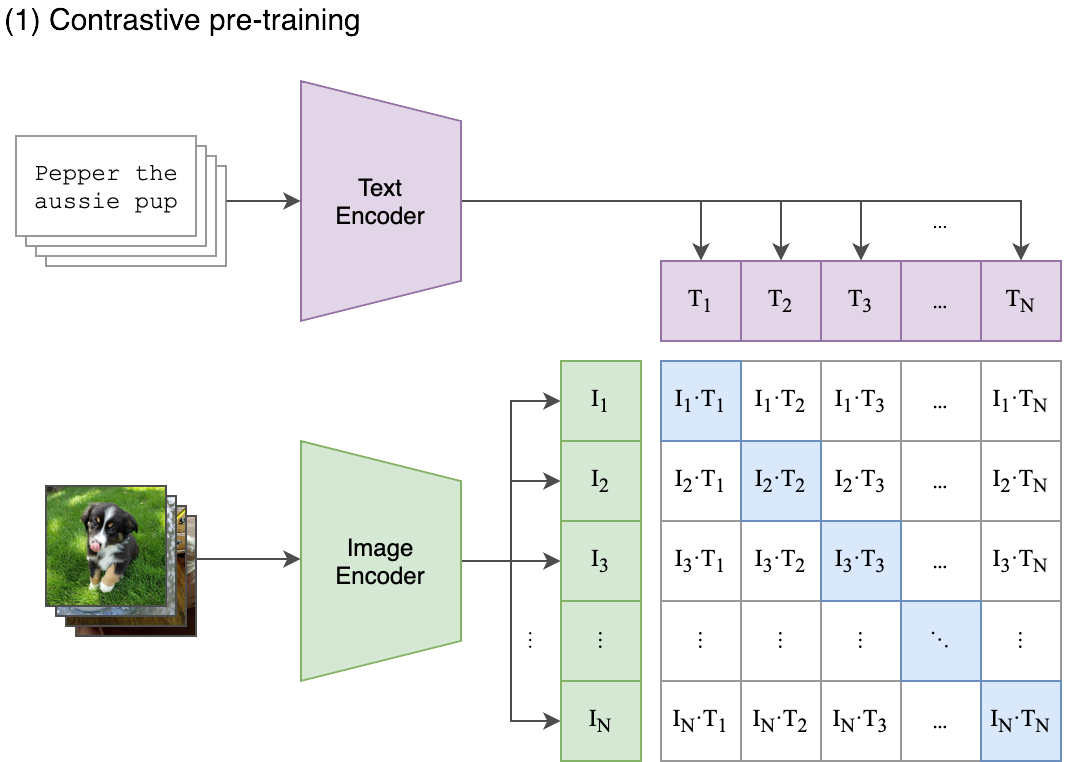
\includegraphics[scale=0.5]{./Slike/CLIP_arhitektura.png}
    \caption{Interakcija slikovnog i tekstualnog kodera CLIP-a. Preuzeto iz~\cite{radford2021learning}.}
    \label{fig:CLIP_architecture}
\end{figure}

\subsection{Okvir učenja}

Kada govorimo o CLIP-u kao okviru učenja, tada govorimo o okviru za multimodalno samonadzirano kontrastno učenje.\ Cilj učenja je naučiti i istovremeno uskladiti ugrađivanja dviju modalnosti.\ 
Kako bismo ovo postigli, prilikom učenja slikovnog i tekstualnog kodera želimo maksimizirati sličnost ugrađivanja slika i njihovih odgovarajućih opisa.\ Dodatno, želimo i minimizirati sličnost ugrađivanja krivo uparenih slika i opisa.\ 
CLIP za učenje ovog zadatka koristi infoNCE gubitak primijenjen dvosmjerno.\ CLIP gubitak možemo prikazati jednadžbom: 

\begin{equation}
    L_{CLIP} = - \frac{1}{2N} \sum_{j=1}^{N} \log{\frac{\exp(\langle z_{j}^I, z_{j}^T \rangle / \tau)}{\sum_{k=1}^{N}{\exp(\langle z_{j}^I, z_{k}^T \rangle / \tau)}}} - \frac{1}{2N} \sum_{k=1}^{N} \log{\frac{\exp(\langle z_{k}^I, z_{k}^T \rangle / \tau)}{\sum_{j=1}^{N}{\exp(\langle z_{j}^I, z_{k}^T \rangle / \tau)}}}
    \label{eq:CLIP_loss}
\end{equation}

Pritom $z_{j}^I$ označava slikovno ugrađivanje slike primjera $x_{j}^I$, $z_{j}^T$ tekstualno ugrađivanje opisa primjera $x_{j}^T$, a $\tau$ parametar temperature.\ 
Kao i prije, oznaka $\langle ... \rangle$ označava skalarni produkt elemenata unutar zagrada.\ 
CLIP gubitak sastoji se od dvije komponente jer želimo imati simetričnu usklađenost ugrađivanja slika i teksta u zajedničkom metričkom prostoru.\

\section{\textit{Zero-shot} učenje}

\textit{Zero-shot} učenje~\cite{xian2018zero} zadatak je dubokog učenja kod kojeg model na ulaz dobiva primjere iz neviđenih razreda te treba predvidjeti njihove oznake tj.\ razrede.\ 
Modeli učeni multimodalnim samonadziranim učenjem poput CLIP-a pogodni su za ovaj zadatak, no zahtijevaju dodatne informacije kako bi ga mogli obavljati.\

Na slici~\ref{fig:CLIP_zero_shot} možemo vidjeti kako se provodi \textit{zero-shot} učenje kod CLIP-a.\ 
Kako bi CLIP mogao predvidjeti jedan od neviđenih razreda, na ulaz tekstualnog kodera dobiva opise u koje su ugrađena imena mogućih razreda.\ 
Za svaki od opisa izračuna se pripadno ugrađivanje te se ono usporedi s ugrađivanjem željene slike.\ Predviđeni razred je onaj za koji je sličnost pripadnog tekstualnog ugrađivanja sa slikovnim ugrađivanjem najveća.\

\begin{figure}[h]
    \centering
    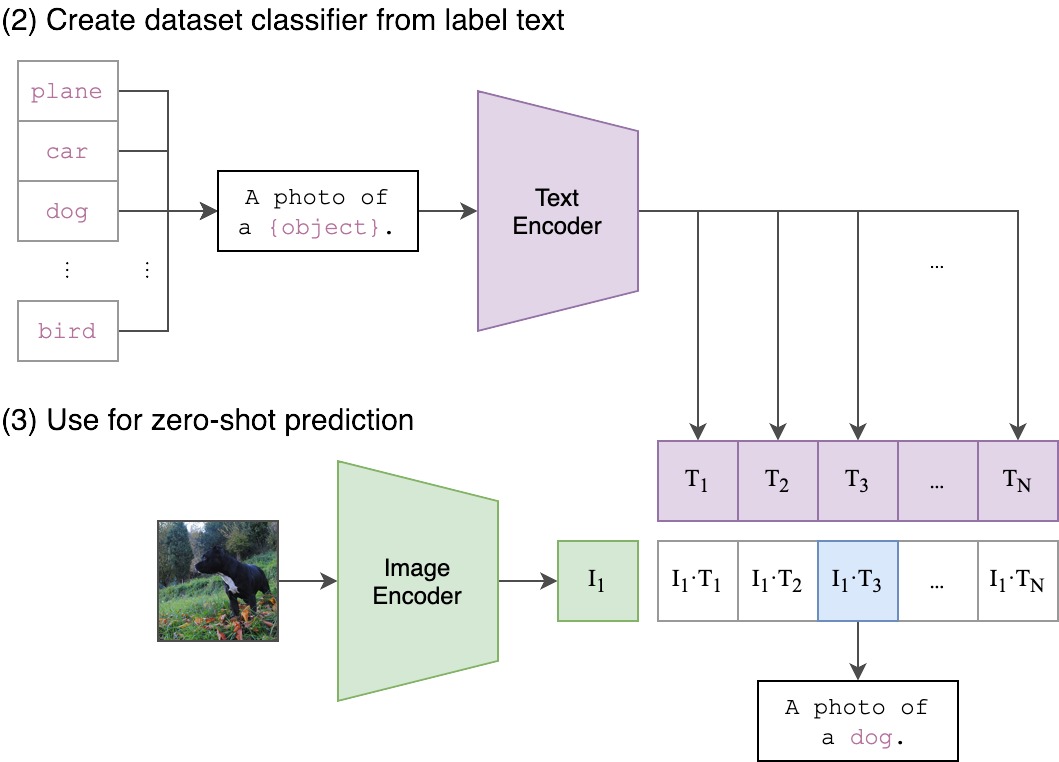
\includegraphics[scale=0.5]{./Slike/CLIP_zero_shot.png}
    \caption{\textit{Zero-shot} učenje kod CLIP-a. Preuzeto iz~\cite{radford2021learning}.}
    \label{fig:CLIP_zero_shot}
\end{figure}

\chapter{Skupovi podataka}

\section{CC3M}

Skup CC3M (engl.\ \textit{Conceptual Captions 3 Million})~\cite{sharma2018conceptual} sastoji se od otprilike 3.3 milijuna slika i pripadnih opisa.\ 
Slike i njihovi opisi prikupljeni su s Interneta, a prikazuju razne scene i objekte iz svakodnevnice.\ Za prikupljanje opisa korišten je \textit{Alt-text} HTML atribut asociran sa slikama na Internetu.\ 
Parovi slika i opisa dodatno su filtrirani i transformirani kako bi se postigla uravnoteženost čistoće, jasnoće i informativnosti opisa.\ Postupak filtriranja i transformiranja u potpunosti je automatiziran.\ 

Na slici~\ref{fig:CC3M} možemo vidjeti dva primjera slika i opisa iz skupa CC3M.\ Dodatno, na slici možemo vidjeti i originalne \textit{Alt-text} HTML atribute na temelju kojih su nastali pripadni opisi.\
Konačni opisi puno sažetije opisuju pripadnu sliku u usporedbi s \textit{Alt-text} HTML atributima.\

\begin{figure}[h]
    \centering
    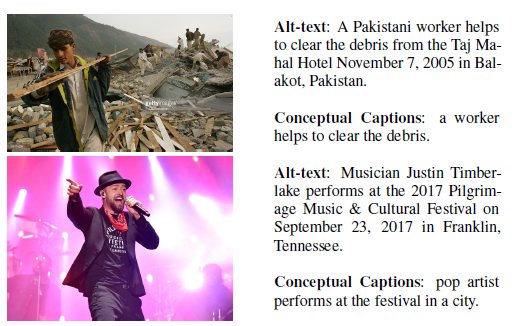
\includegraphics[scale=0.7]{./Slike/CC3M.png}
    \caption{Primjer slika i opisa iz skupa CC3M. Preuzeto iz~\cite{sharma2018conceptual}.}
    \label{fig:CC3M}
\end{figure}

\section{ImageNet1K}

Skup ImageNet1K najčešće je korišteni podskup skupa ImageNet~\cite{deng2009imagenet}.\ 
Podijeljen je na 1 281 167 slika u skupu za učenje, 50 000 slika u skupu za validaciju i 100 000 slika u skupu za ispitivanje.\ 
Svaka od slika može pripadati jednom od ukupno 1000 razreda.\ Pojedini razredi predstavljaju različite koncepte, od životinja pa sve do različitih vrsta igračaka.\ 
Podskup ImageNet1K godinama se koristio za evaluaciju algoritama za klasifikaciju i detekciju objekata u sklopu natjecanja ILSVRC (engl.\ \textit{mageNet Large Scale Visual Recognition Challenge}).\
  
Slika~\ref{fig:imagenet} prikazuje nekoliko slika i razreda iz skupa ImageNet.\ Skup podataka strukturiran je hijerarhijski.\ Slike iz razreda \texttt{husky} također pripadaju i u razrede \texttt{dog} te \texttt{mammal}.\

\begin{figure}[h]
    \centering
    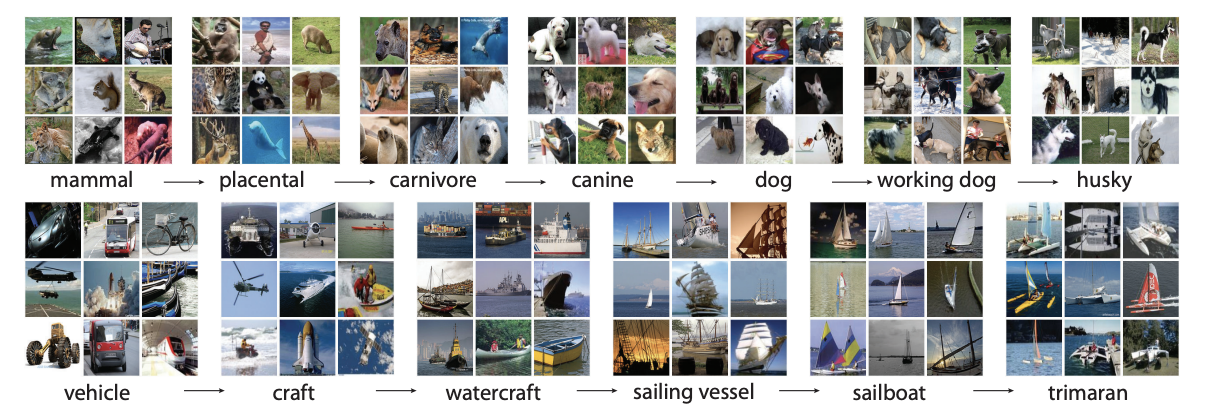
\includegraphics[scale=0.33]{./Slike/imagenet.png}
    \caption{Primjer slika i razreda iz skupa ImageNet. Preuzeto iz~\cite{deng2009imagenet}.}
    \label{fig:imagenet}
\end{figure}

\chapter{Zaključak}
Zaključak.

\bibliography{literatura}
\bibliographystyle{fer}

\chapter{Sažetak}
Sažetak.

\end{document}
